\pagebreak
\section*{6. Application-Specific Integrated Circuit}
\addcontentsline{toc}{chapter}{Application-Specific Integrated Circuit}

An application-specific integrated circuit (ASIC) is an integrated circuit (IC) chip customized for a particular use, rather than intended for general-purpose use. For example, a chip designed to run in a digital voice recorder or a high-efficiency bitcoin miner is an ASIC. Application-specific standard product (ASSP) chips are intermediate between ASICs and industry standard integrated circuits like the 7400 series or the 4000 series. ASIC chips are typically fabricated using metal-oxide-semiconductor (MOS) technology, as MOS integrated circuit chips.\vspace{.3cm}

As feature sizes have shrunk and design tools improved over the years, the maximum complexity (and hence functionality) possible in an ASIC has grown from 5,000 logic gates to over 100 million. Modern ASICs often include entire microprocessors, memory blocks including ROM, RAM, EEPROM, flash memory and other large building blocks. Such an ASIC is often termed a SoC (system-on-chip). Designers of digital ASICs often use a hardware description language (HDL), such as Verilog or VHDL, to describe the functionality of ASICs.\vspace{.3cm}

Field-programmable gate arrays (FPGA) are the modern-day technology for building a breadboard or prototype from standard parts[vague]; programmable logic blocks and programmable interconnects allow the same FPGA to be used in many different applications. For smaller designs or lower production volumes, FPGAs may be more cost-effective than an ASIC design, even in production. The non-recurring engineering (NRE) cost of an ASIC can run into the millions of dollars. Therefore, device manufacturers typically prefer FPGAs for prototyping and devices with low production volume and ASICs for very large production volumes where NRE costs can be amortized across many devices.\vspace{.3cm}

\begin{figure}[h]
	\centering
	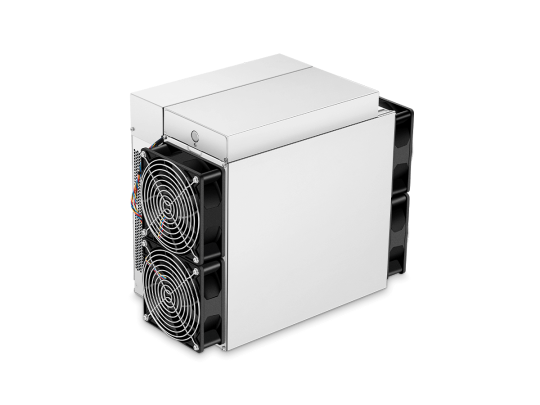
\includegraphics[width=0.7\linewidth]{images/176bd485-ad85-44f7-b60b-cdcbd32de623_540}
	\captionsetup{labelformat=empty}
	\caption{Application-Specific Integrated Circuit}
\end{figure}

\subsection*{6.1 History}
Early ASICs used gate array technology. By 1967, Ferranti and Interdesign were manufacturing early bipolar gate arrays. In 1967, Fairchild Semiconductor introduced the Micromatrix family of bipolar diode–transistor logic (DTL) and transistor–transistor logic (TTL) arrays.\vspace{.3cm}

Complementary metal-oxide-semiconductor (CMOS) technology opened the door to the broad commercialization of gate arrays. The first CMOS gate arrays were developed by Robert Lipp,[3][4] in 1974 for International Microcircuits, Inc. (IMI).\vspace{.3cm}

Metal-oxide-semiconductor (MOS) standard cell technology was introduced by Fairchild and Motorola, under the trade names Micromosaic and Polycell, in the 1970s. This technology was later successfully commercialized by VLSI Technology (founded 1979) and LSI Logic (1981).\vspace{.3cm}

A successful commercial application of gate array circuitry was found in the low-end 8-bit ZX81 and ZX Spectrum personal computers, introduced in 1981 and 1982. These were used by Sinclair Research (UK) essentially as a low-cost I/O solution aimed at handling the computer's graphics.\vspace{.3cm}

Customization occurred by varying a metal interconnect mask. Gate arrays had complexities of up to a few thousand gates; this is now called mid-scale integration. Later versions became more generalized, with different base dies customized by both metal and polysilicon layers. Some base dies also include random-access memory (RAM) elements.\vspace{.3cm}